%% March 2018
%%%%%%%%%%%%%%%%%%%%%%%%%%%%%%%%%%%%%%%%%%%%%%%%%%%%%%%%%%%%%%%%%%%%%%%%%%%%
% AGUJournalTemplate.tex: this template file is for articles formatted with LaTeX
%
% This file includes commands and instructions
% given in the order necessary to produce a final output that will
% satisfy AGU requirements, including customized APA reference formatting.
%
% You may copy this file and give it your
% article name, and enter your text.
%
%
% Step 1: Set the \documentclass
%
% There are two options for article format:
%
% PLEASE USE THE DRAFT OPTION TO SUBMIT YOUR PAPERS.
% The draft option produces double spaced output.
%

%% To submit your paper:
\documentclass[draft]{agujournal2018}
\usepackage{apacite}
\usepackage{url} %this package should fix any errors with URLs in refs.
%%%%%%%
% As of 2018 we recommend use of the TrackChanges package to mark revisions.
% The trackchanges package adds five new LaTeX commands:
%
%  \note[editor]{The note}
%  \annote[editor]{Text to annotate}{The note}
%  \add[editor]{Text to add}
%  \remove[editor]{Text to remove}
%  \change[editor]{Text to remove}{Text to add}
%
% complete documentation is here: http://trackchanges.sourceforge.net/
%%%%%%%


%% Enter journal name below.
%% Choose from this list of Journals:
%
% JGR: Atmospheres
% JGR: Biogeosciences
% JGR: Earth Surface
% JGR: Oceans
% JGR: Planets
% JGR: Solid Earth
% JGR: Space Physics
% Global Biogeochemical Cycles
% Geophysical Research Letters
% Paleoceanography and Paleoclimatology
% Radio Science
% Reviews of Geophysics
% Tectonics
% Space Weather
% Water Resources Research
% Geochemistry, Geophysics, Geosystems
% Journal of Advances in Modeling Earth Systems (JAMES)
% Earth's Future
% Earth and Space Science
% Geohealth
%
% ie, \journalname{Water Resources Research}

\journalname{JGR: Machine Learning and Computation}


% tightlist command for lists without linebreak
\providecommand{\tightlist}{%
  \setlength{\itemsep}{0pt}\setlength{\parskip}{0pt}}

% From pandoc table feature
\usepackage{longtable,booktabs,array}
\usepackage{calc} % for calculating minipage widths
% Correct order of tables after \paragraph or \subparagraph
\usepackage{etoolbox}
\makeatletter
\patchcmd\longtable{\par}{\if@noskipsec\mbox{}\fi\par}{}{}
\makeatother
% Allow footnotes in longtable head/foot
\IfFileExists{footnotehyper.sty}{\usepackage{footnotehyper}}{\usepackage{footnote}}
\makesavenoteenv{longtable}


\usepackage{pdflscape}
\newcommand{\blandscape}{\begin{landscape}}
\newcommand{\elandscape}{\end{landscape}}
\usepackage{longtable}
\usepackage{tabularx}
\usepackage{booktabs}
\usepackage{setspace}
\usepackage{caption}
\captionsetup[figure]{font={stretch=0.6}}
\usepackage{float}
\raggedbottom
\usepackage{soul}
\usepackage[utf8]{inputenc}
\usepackage{amsmath}
\usepackage{amsfonts}
\usepackage{amssymb}
\DeclareUnicodeCharacter{2212}{-}
\DeclareUnicodeCharacter{02DA}{$^\circ$}
\DeclareUnicodeCharacter{2265}{$\geq$}
\DeclareUnicodeCharacter{2264}{$\leq$}
\DeclareUnicodeCharacter{177}{$\pm$}
\providecommand{\tightlist}{\setlength{\itemsep}{0pt}\setlength{\parskip}{0pt}}
\def\tightlist{}
\usepackage{hyperref}
\renewcommand\thefigure{S\arabic{figure}}
\renewcommand\thetable{S\arabic{table}}
\usepackage{booktabs}
\usepackage{longtable}
\usepackage{array}
\usepackage{multirow}
\usepackage{wrapfig}
\usepackage{float}
\usepackage{colortbl}
\usepackage{pdflscape}
\usepackage{tabu}
\usepackage{threeparttable}
\usepackage{threeparttablex}
\usepackage[normalem]{ulem}
\usepackage{makecell}
\usepackage{xcolor}

\begin{document}


%% ------------------------------------------------------------------------ %%
%  Title
%
% (A title should be specific, informative, and brief. Use
% abbreviations only if they are defined in the abstract. Titles that
% start with general keywords then specific terms are optimized in
% searches)
%
%% ------------------------------------------------------------------------ %%

% Example: \title{This is a test title}

\title{Supporting Information for RocMLMs: Predicting Rock Properties through Machine Learning Models}

%% ------------------------------------------------------------------------ %%
%
%  AUTHORS AND AFFILIATIONS
%
%% ------------------------------------------------------------------------ %%

% Authors are individuals who have significantly contributed to the
% research and preparation of the article. Group authors are allowed, if
% each author in the group is separately identified in an appendix.)

% List authors by first name or initial followed by last name and
% separated by commas. Use \affil{} to number affiliations, and
% \thanks{} for author notes.
% Additional author notes should be indicated with \thanks{} (for
% example, for current addresses).

% Example: \authors{A. B. Author\affil{1}\thanks{Current address, Antartica}, B. C. Author\affil{2,3}, and D. E.
% Author\affil{3,4}\thanks{Also funded by Monsanto.}}

\authors{
Buchanan Kerswell
\affil{1}
Nestor Cerpa
\affil{1}
Andréa Tommasi
\affil{1}
Marguerite Godard
\affil{1}
José Alberto Padrón-Navarta
\affil{2}
}


% \affiliation{1}{First Affiliation}
% \affiliation{2}{Second Affiliation}
% \affiliation{3}{Third Affiliation}
% \affiliation{4}{Fourth Affiliation}

\affiliation{1}{Geosciences Montpellier, University of Montpellier, CNRS, University of Antilles, Place Eugène Bataillon, 34095 Montpellier, France}
\affiliation{2}{Instituto Andaluz de Ciencias de la Tierra (IACT), CSIC, Avda. de las Palmeras, 4, 18100 Armilla (Granada), Spain}
%(repeat as many times as is necessary)

%% Corresponding Author:
% Corresponding author mailing address and e-mail address:

% (include name and email addresses of the corresponding author.  More
% than one corresponding author is allowed in this LaTeX file and for
% publication; but only one corresponding author is allowed in our
% editorial system.)

% Example: \correspondingauthor{First and Last Name}{email@address.edu}
\correspondingauthor{Buchanan Kerswell}{\href{mailto:buchanan.kerswell@umontpellier.fr}{\nolinkurl{buchanan.kerswell@umontpellier.fr}}}

%% Keypoints, final entry on title page.

%  List up to three key points (at least one is required)
%  Key Points summarize the main points and conclusions of the article
%  Each must be 100 characters or less with no special characters or punctuation

% Example:
% \begin{keypoints}
% \item	List up to three key points (at least one is required)
% \item	Key Points summarize the main points and conclusions of the article
% \item	Each must be 100 characters or less with no special characters or punctuation
% \end{keypoints}


%% ------------------------------------------------------------------------ %%
%
%  ABSTRACT
%
% A good abstract will begin with a short description of the problem
% being addressed, briefly describe the new data or analyses, then
% briefly states the main conclusion(s) and how they are supported and
% uncertainties.
%% ------------------------------------------------------------------------ %%

%% \begin{abstract} starts the second page

\section*{Contents of this File}\label{contents-of-this-file}
\addcontentsline{toc}{section}{Contents of this File}

\begin{enumerate}
\def\labelenumi{\arabic{enumi}.}
\tightlist
\item
  Figures \ref{fig:earthchem-harker-diagram} to \ref{fig:image12-PUM-NN3}
\item
  Tables S1
\end{enumerate}

\clearpage

\section*{Synthetic Peridotite Compositions}\label{synthetic-peridotite-compositions}
\addcontentsline{toc}{section}{Synthetic Peridotite Compositions}

Figure \ref{fig:earthchem-harker-diagram} shows a comparison between natural peridotite compositions in the standardized Earthchem.org dataset and synthetic peridotite compositions sampled randomly along the PCA mixing array as described in Section 2.1.2 of the main text. The data in Figure \ref{fig:earthchem-harker-diagram} are the same as presented in Figure 2 of the main text, but show peridotite compositions in chemical space (Harker diagrams vs.~SiO\(_2\)) instead of PC space. The trend from more fertile lherzolite samples to more depleted harzburgite samples is closely approximated by the synthetic peridotite mixing array. While PUM and DMM are often represented in the literature as distinct mantle end-members, they have quite similar major oxide compositions (e.g., Al\(_2\)O\(_3\), CaO, MgO, and FeO). Synthetic mantle end-members PSUM and DSUM represent a much wider range of recorded mantle compositions than PUM and DMM (Figure \ref{fig:earthchem-harker-diagram}).



\begin{figure}[htbp]

{\centering 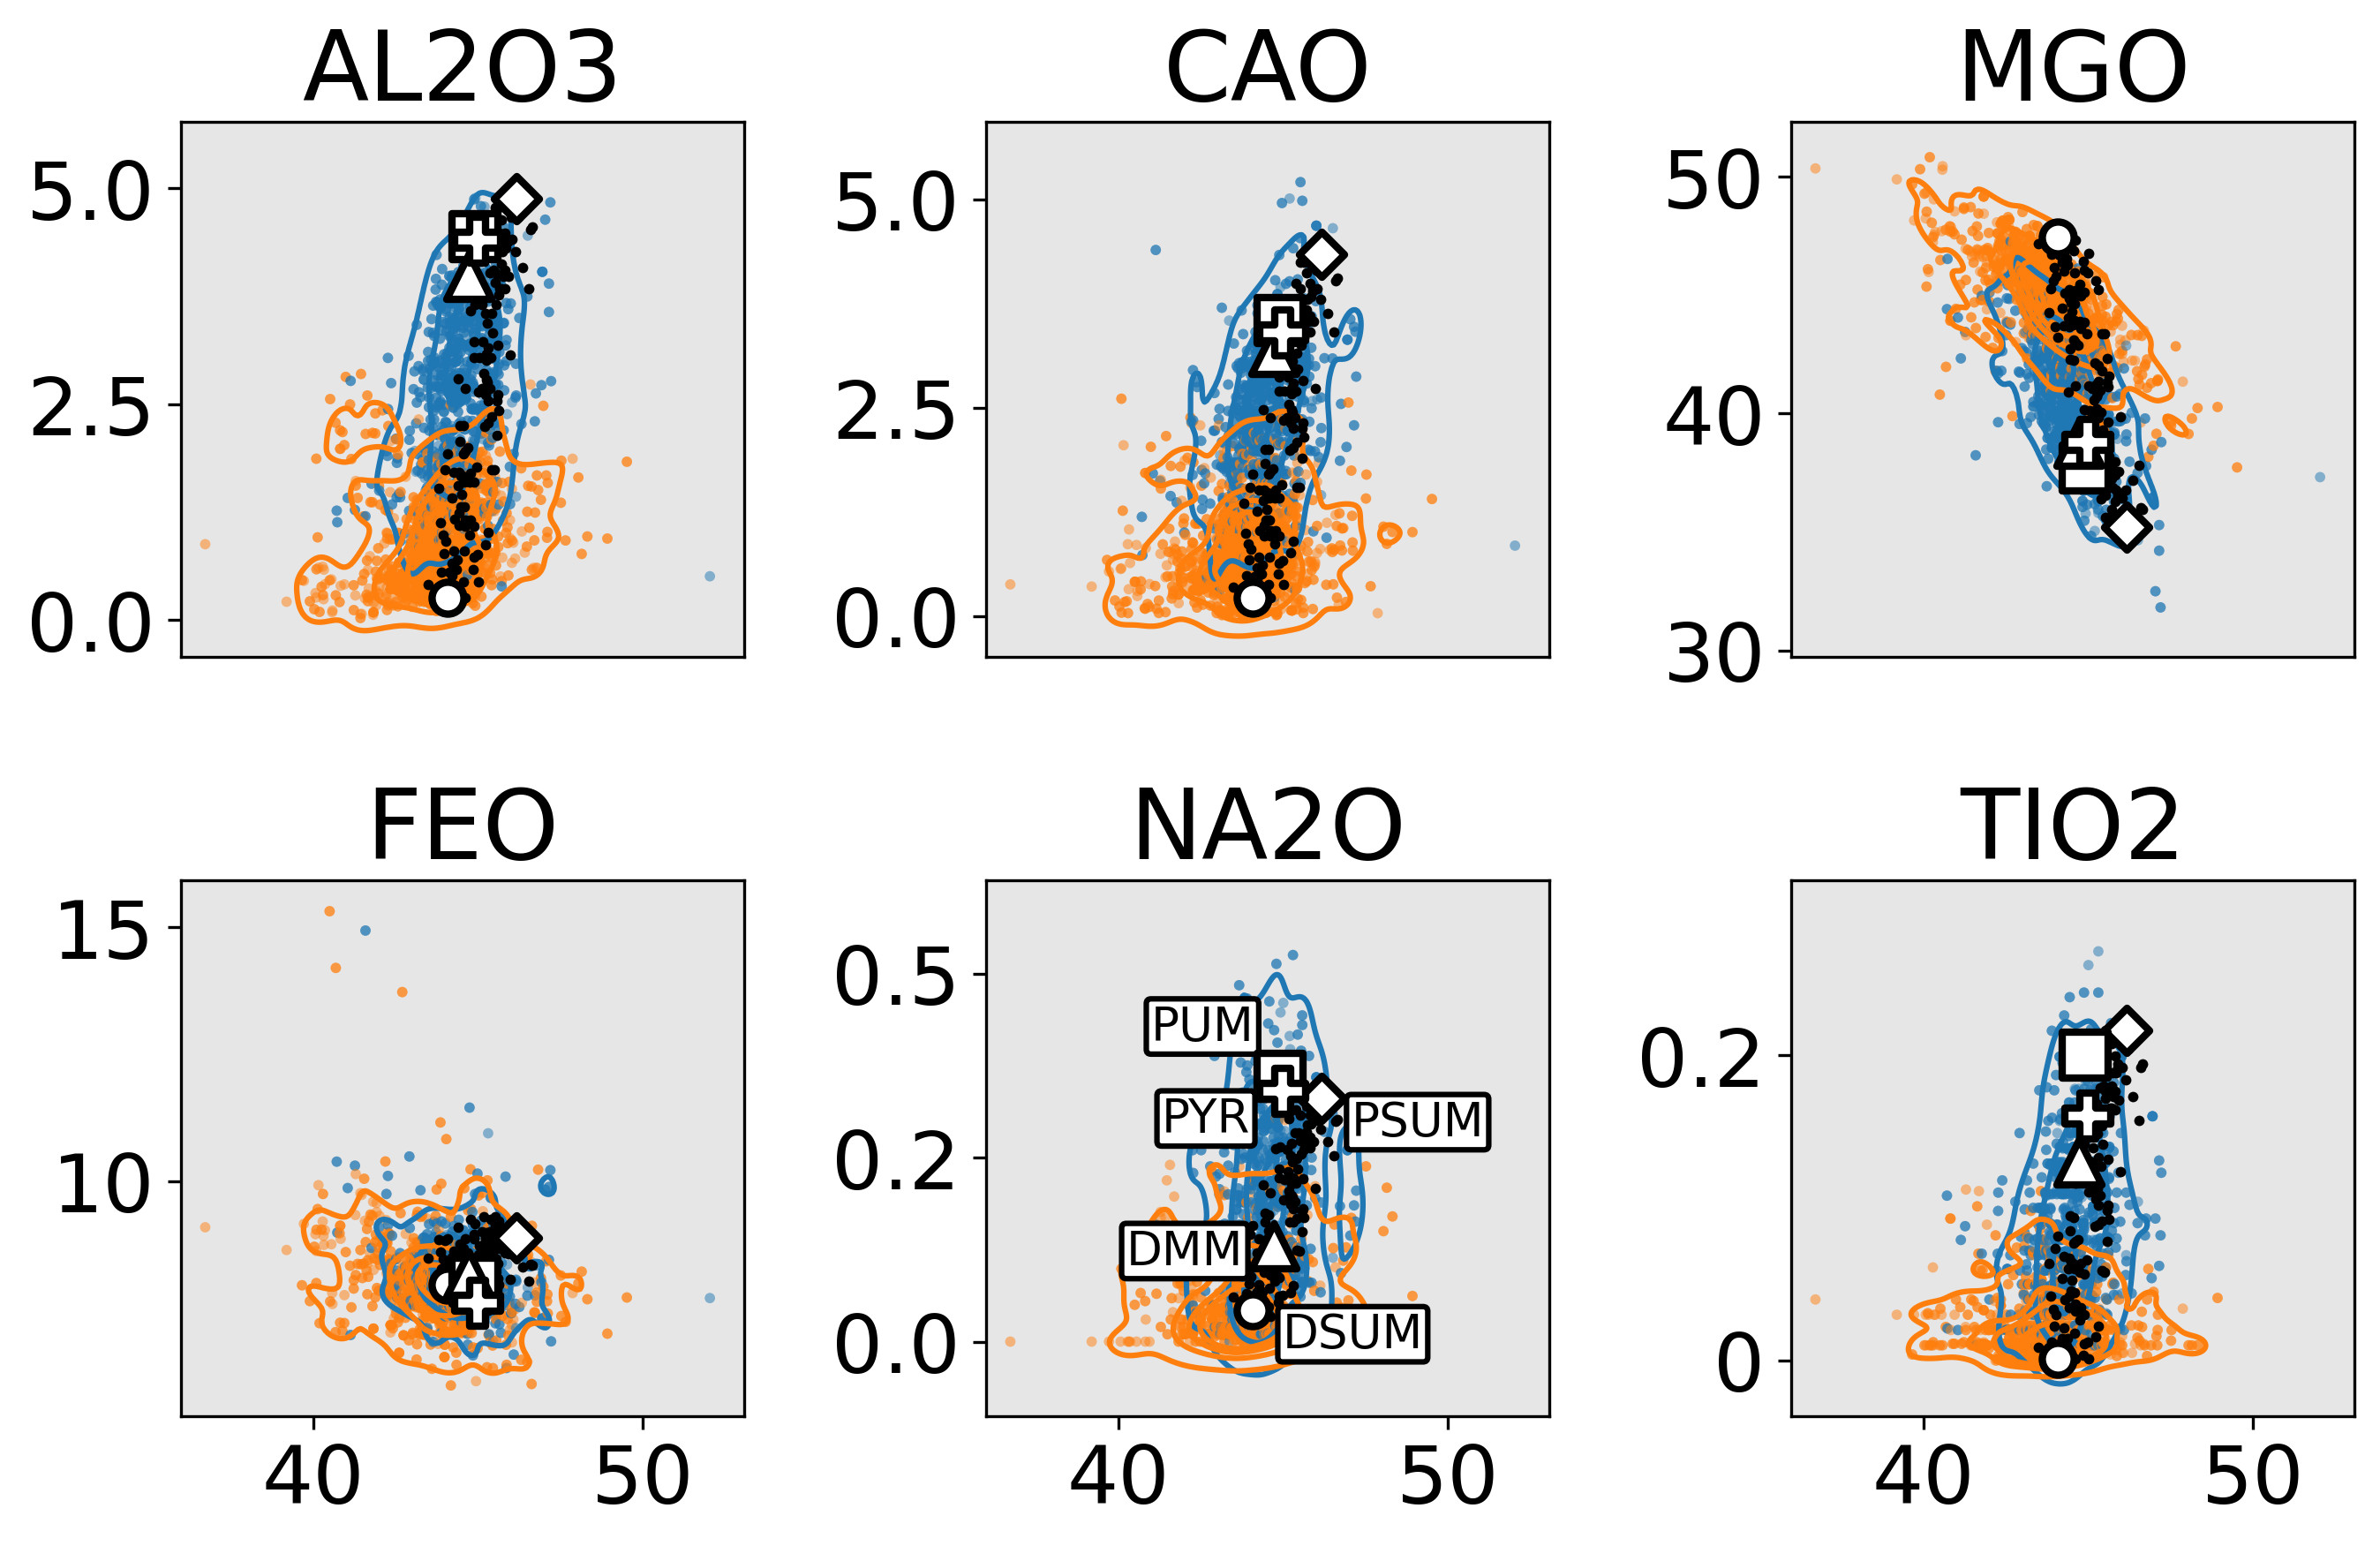
\includegraphics[width=1\linewidth,]{earthchem-harker-diagram} 

}

\caption{Harker Diagrams vs.~SIO2 (in wt.\%) showing the distribution of peridotite samples from Earthchem.org (colored data points and contours). PUM (white square), DMM (white triangle), and pyrolite (white plus) are commonly-referenced bulk mantle compositions (see Table 2 in the main text), while PSUM (white diamond) and DSUM (white circle) define a mixing array used to generate RocMLM training data (black data points).}\label{fig:earthchem-harker-diagram}
\end{figure}

\clearpage

\section*{RocMLM Regression Algorithms}\label{rocmlm-regression-algorithms}
\addcontentsline{toc}{section}{RocMLM Regression Algorithms}

Figures \ref{fig:image12-PUM-DT}--\ref{fig:image12-PUM-NN3} show RocMLM predictions and depth profiles for a PUM bulk mantle composition. The Decision Tree, single-layer Neural Network, and three-layer Neural Network RocMLMs were presented in the main text (Figures 3--5), while the k-Neighbors (Figure \ref{fig:image12-PUM-KN}) and two-layer Neural Network RocMLMs (Figures \ref{fig:image12-PUM-NN2}) are presented here for a comprehensive comparison of all the regression algorithms tested in this study.



\begin{figure}[htbp]

{\centering 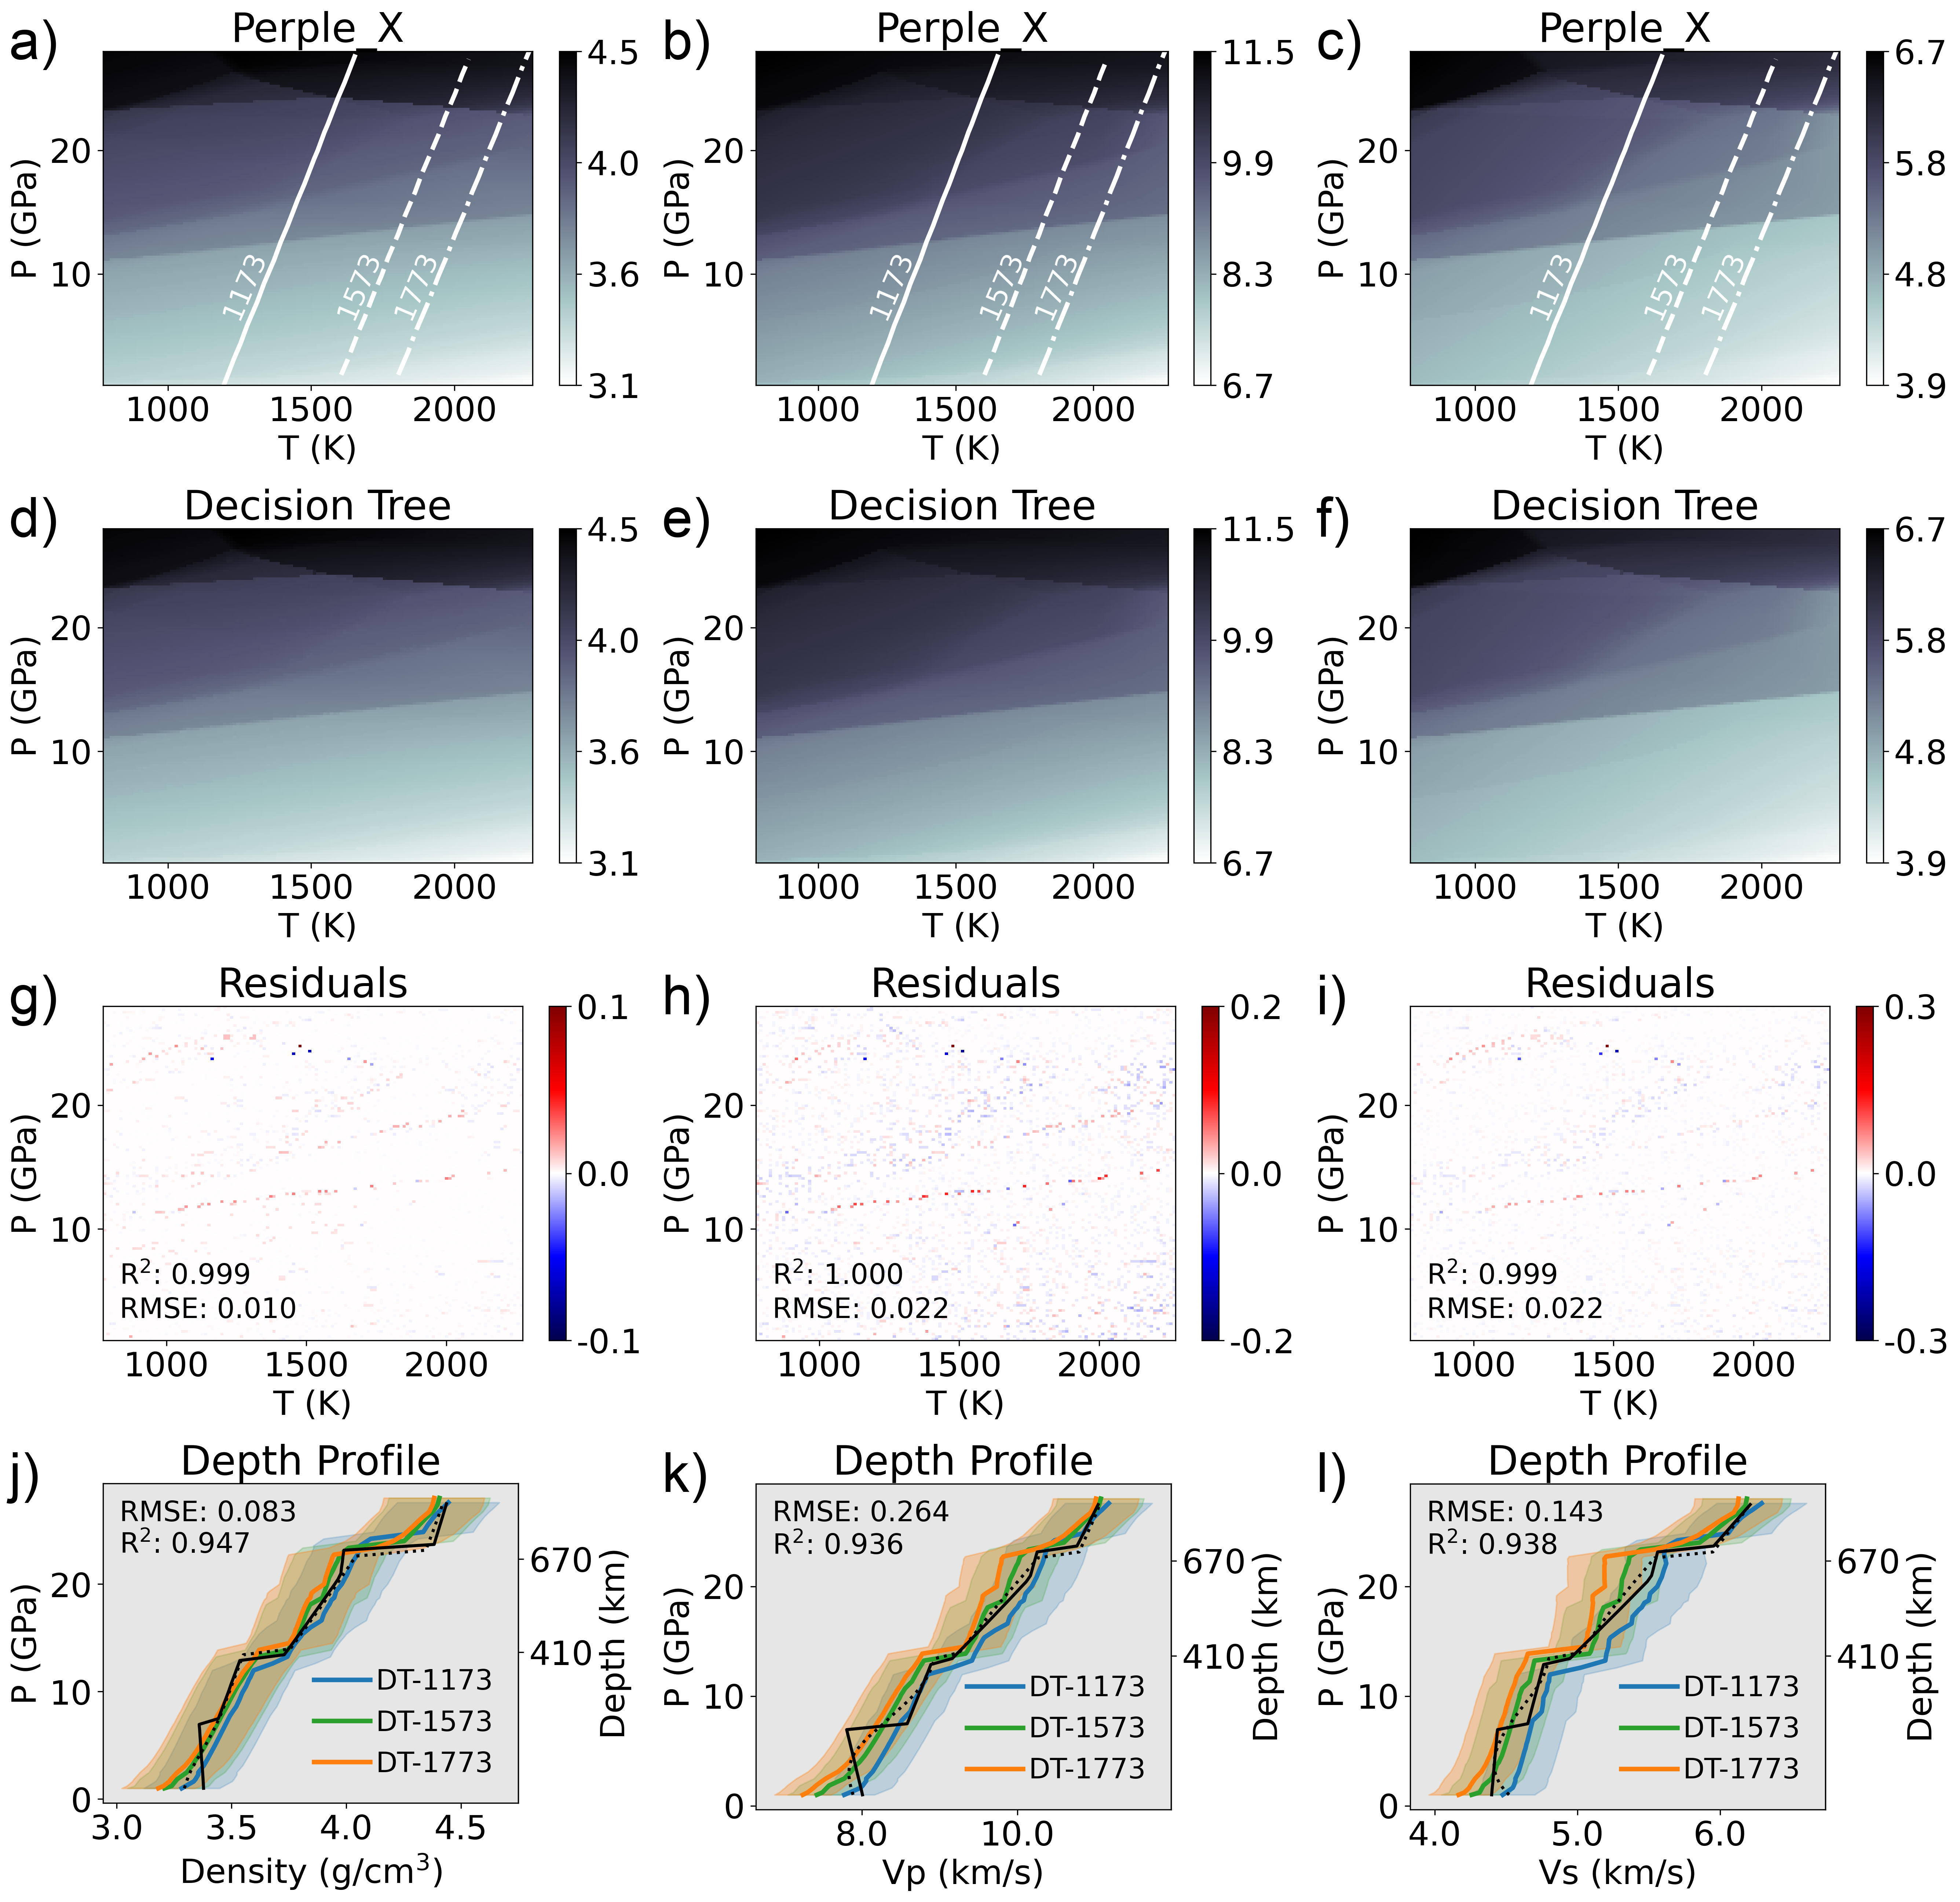
\includegraphics[width=1\linewidth,]{image12-PUM-DT} 

}

\caption{(ref:image12-PUM-DT-cap)}\label{fig:image12-PUM-DT}
\end{figure}



\begin{figure}[htbp]

{\centering 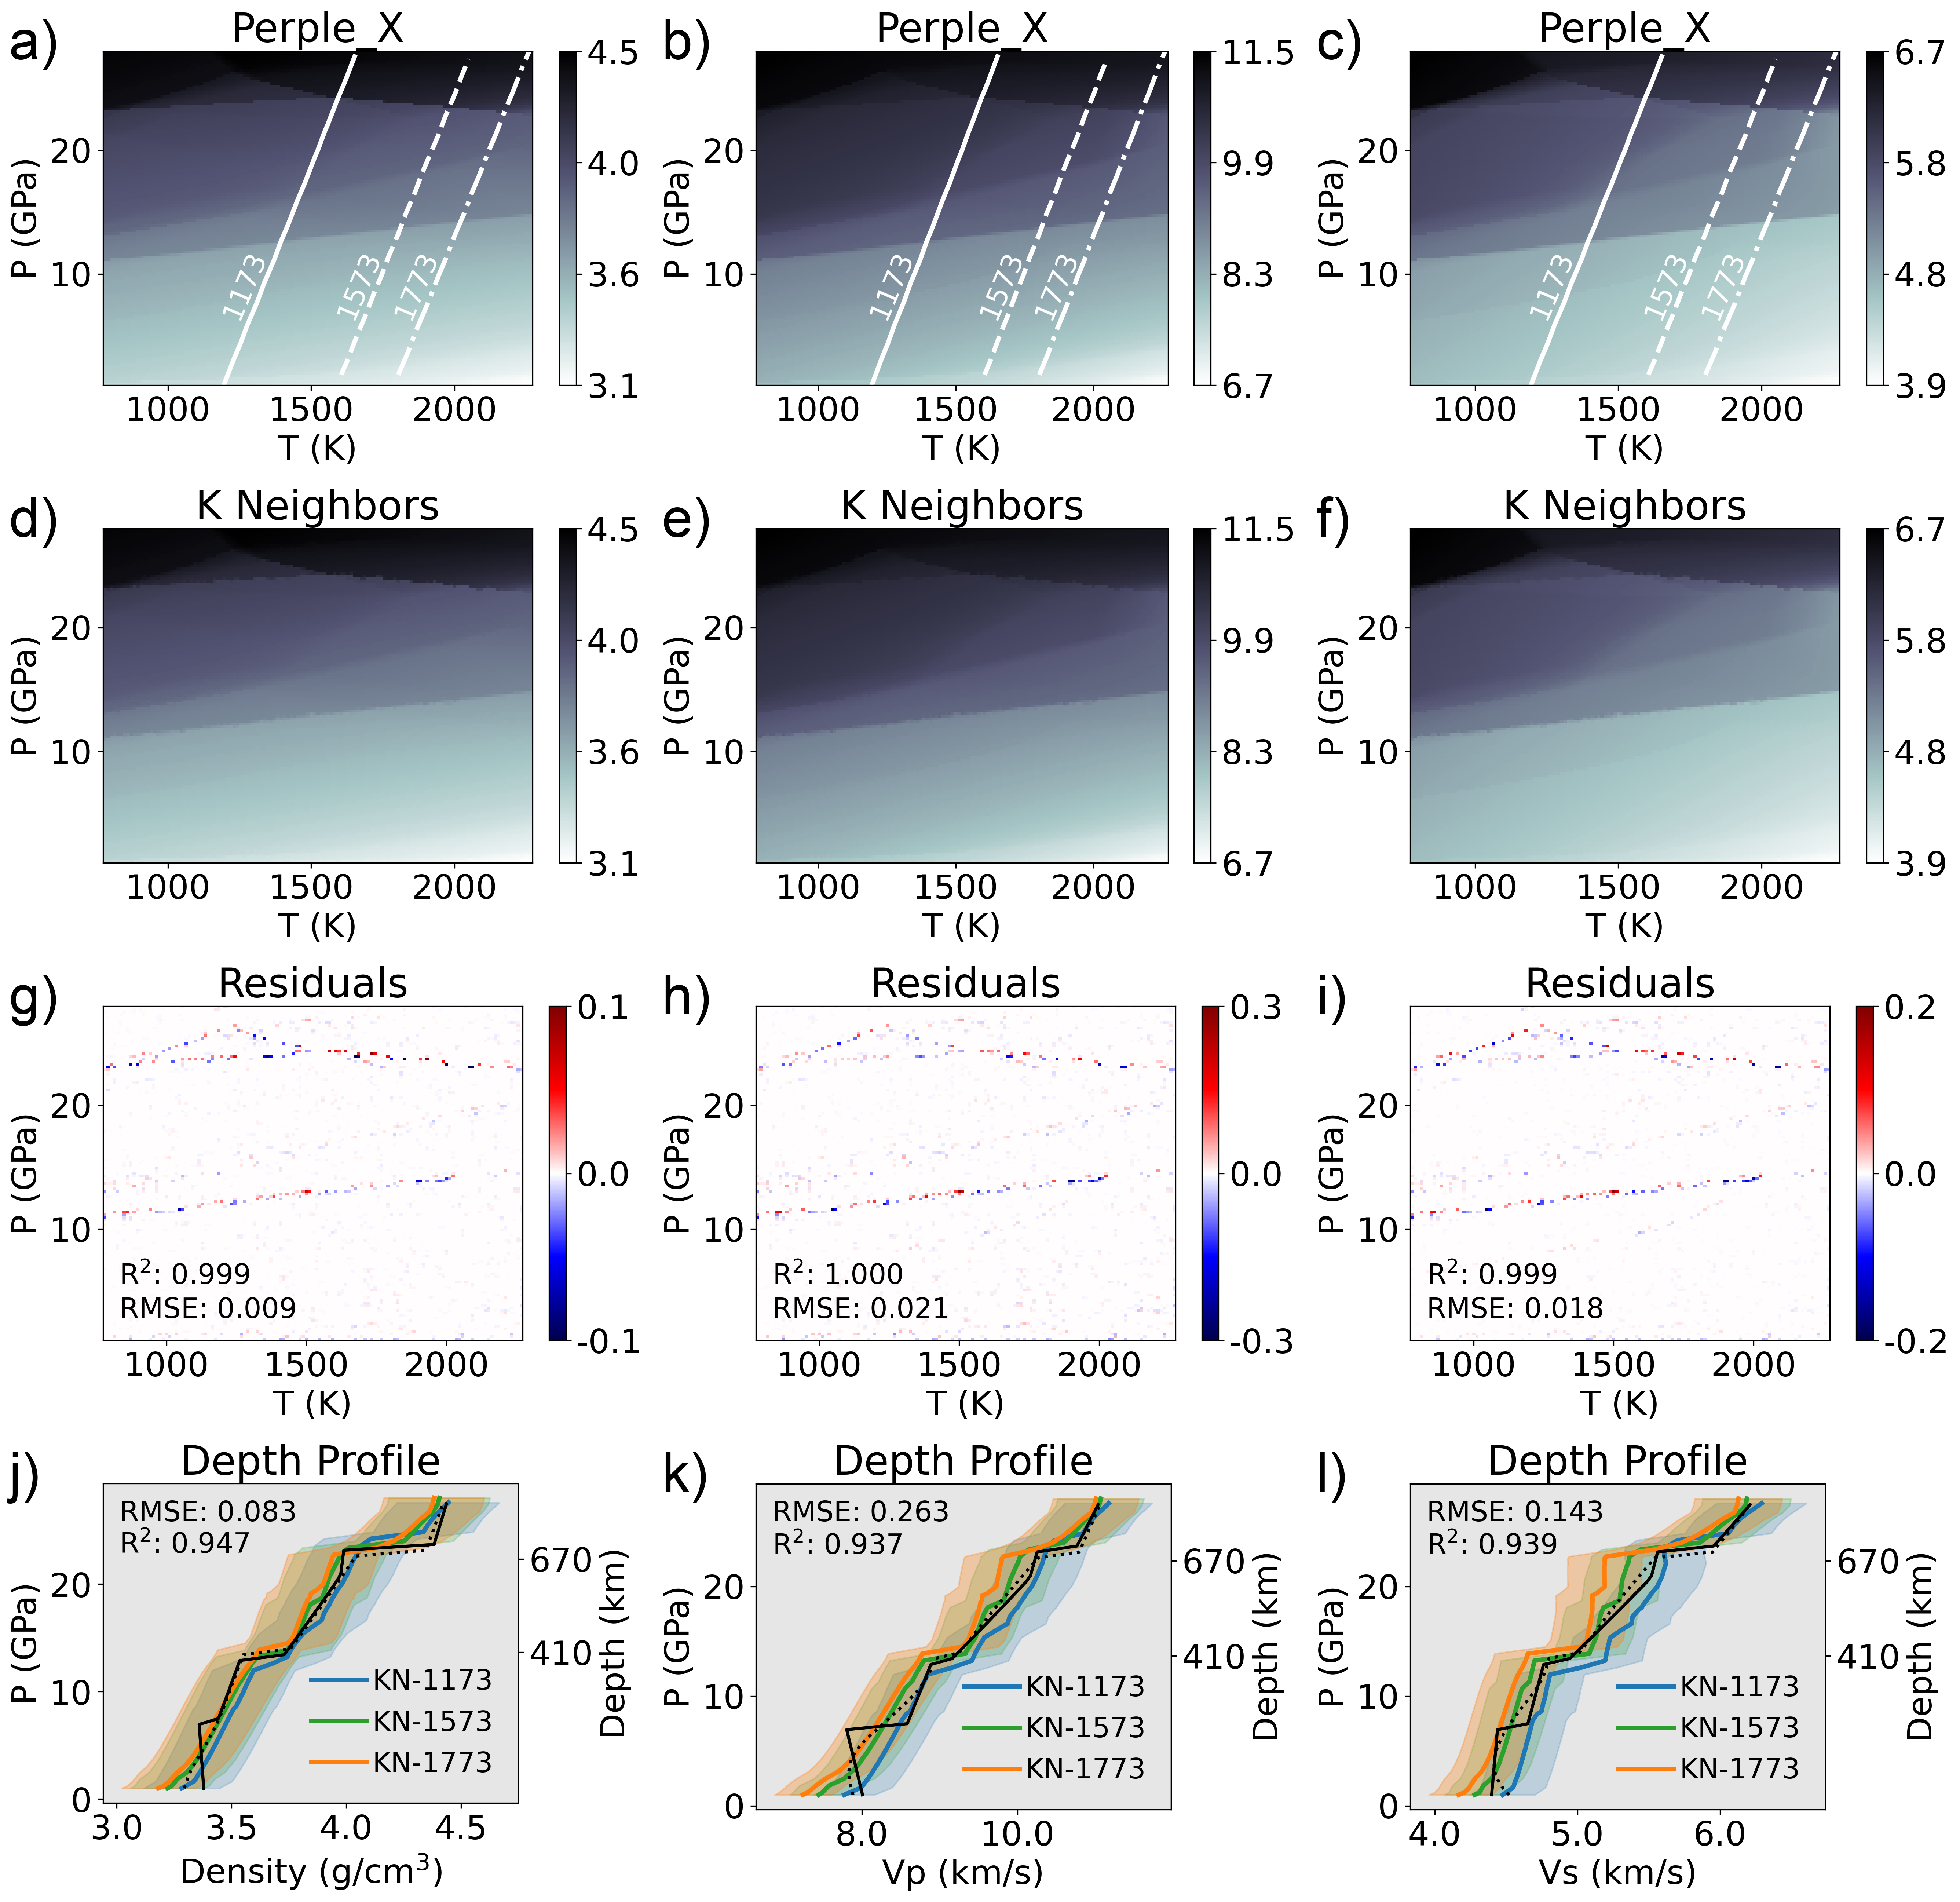
\includegraphics[width=1\linewidth,]{image12-PUM-KN} 

}

\caption{(ref:image12-PUM-KN-cap)}\label{fig:image12-PUM-KN}
\end{figure}



\begin{figure}[htbp]

{\centering 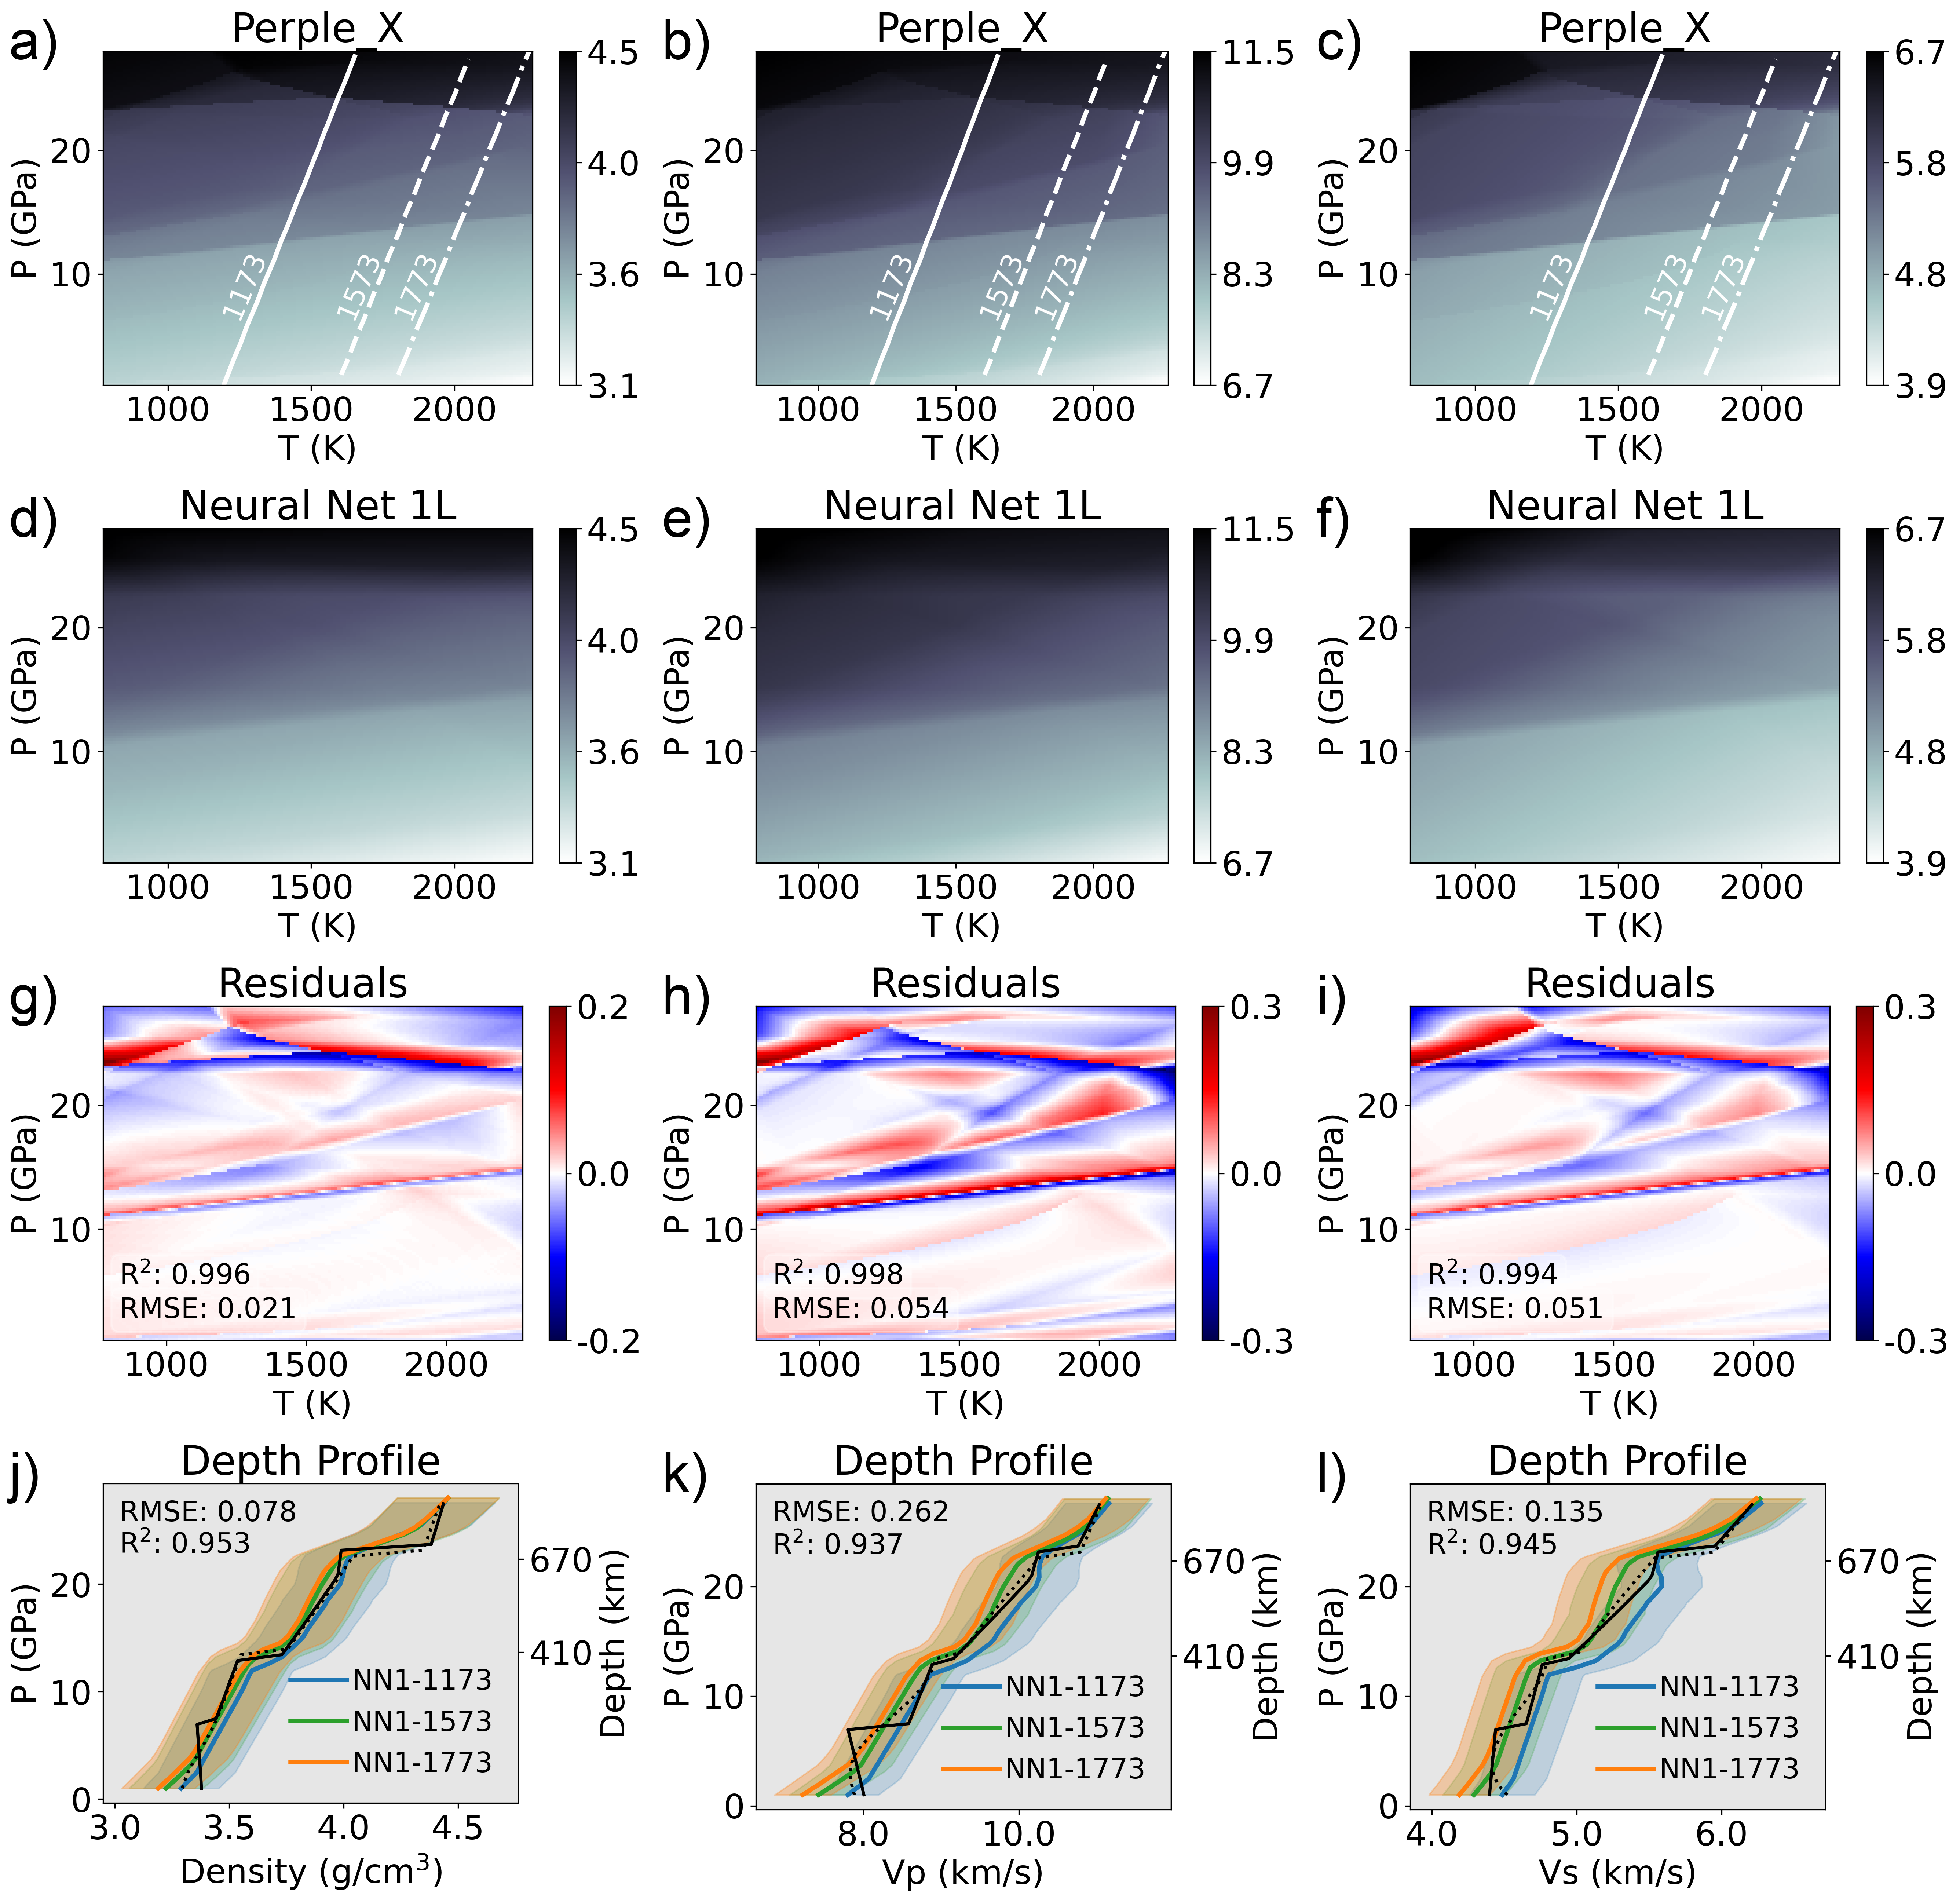
\includegraphics[width=1\linewidth,]{image12-PUM-NN1} 

}

\caption{(ref:image12-PUM-NN1-cap)}\label{fig:image12-PUM-NN1}
\end{figure}



\begin{figure}[htbp]

{\centering 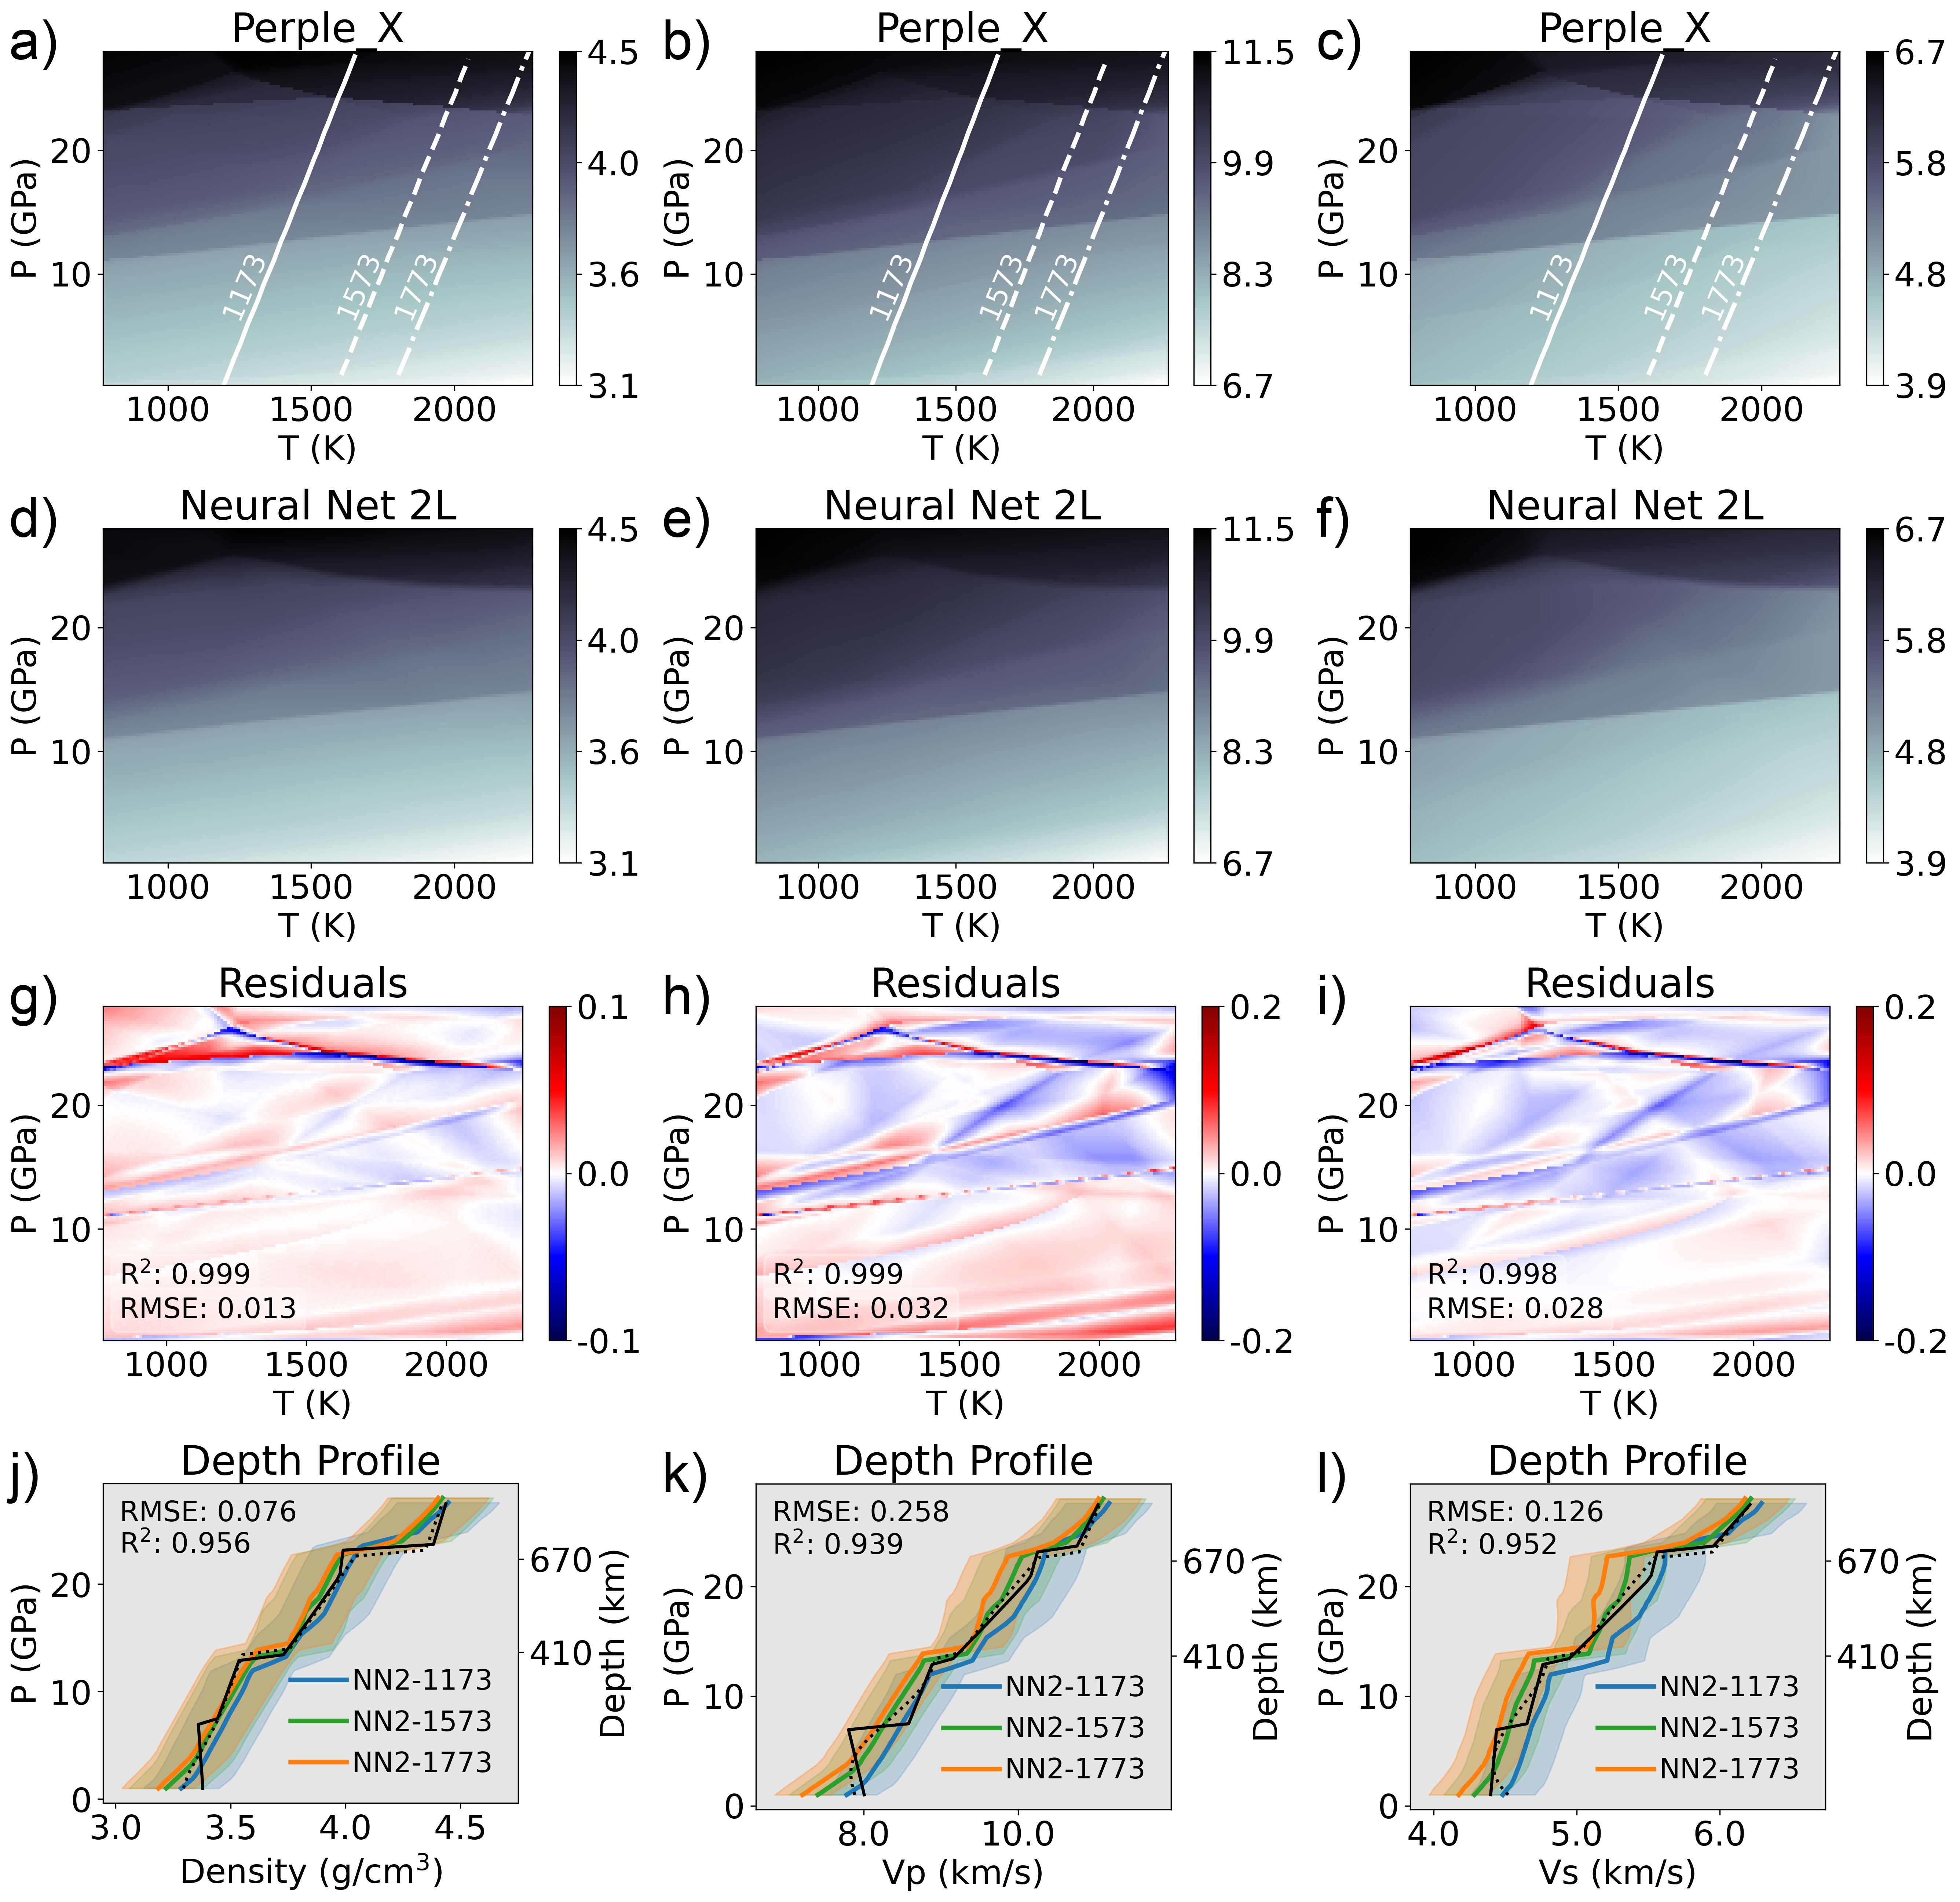
\includegraphics[width=1\linewidth,]{image12-PUM-NN2} 

}

\caption{(ref:image12-PUM-NN2-cap)}\label{fig:image12-PUM-NN2}
\end{figure}



\begin{figure}[htbp]

{\centering 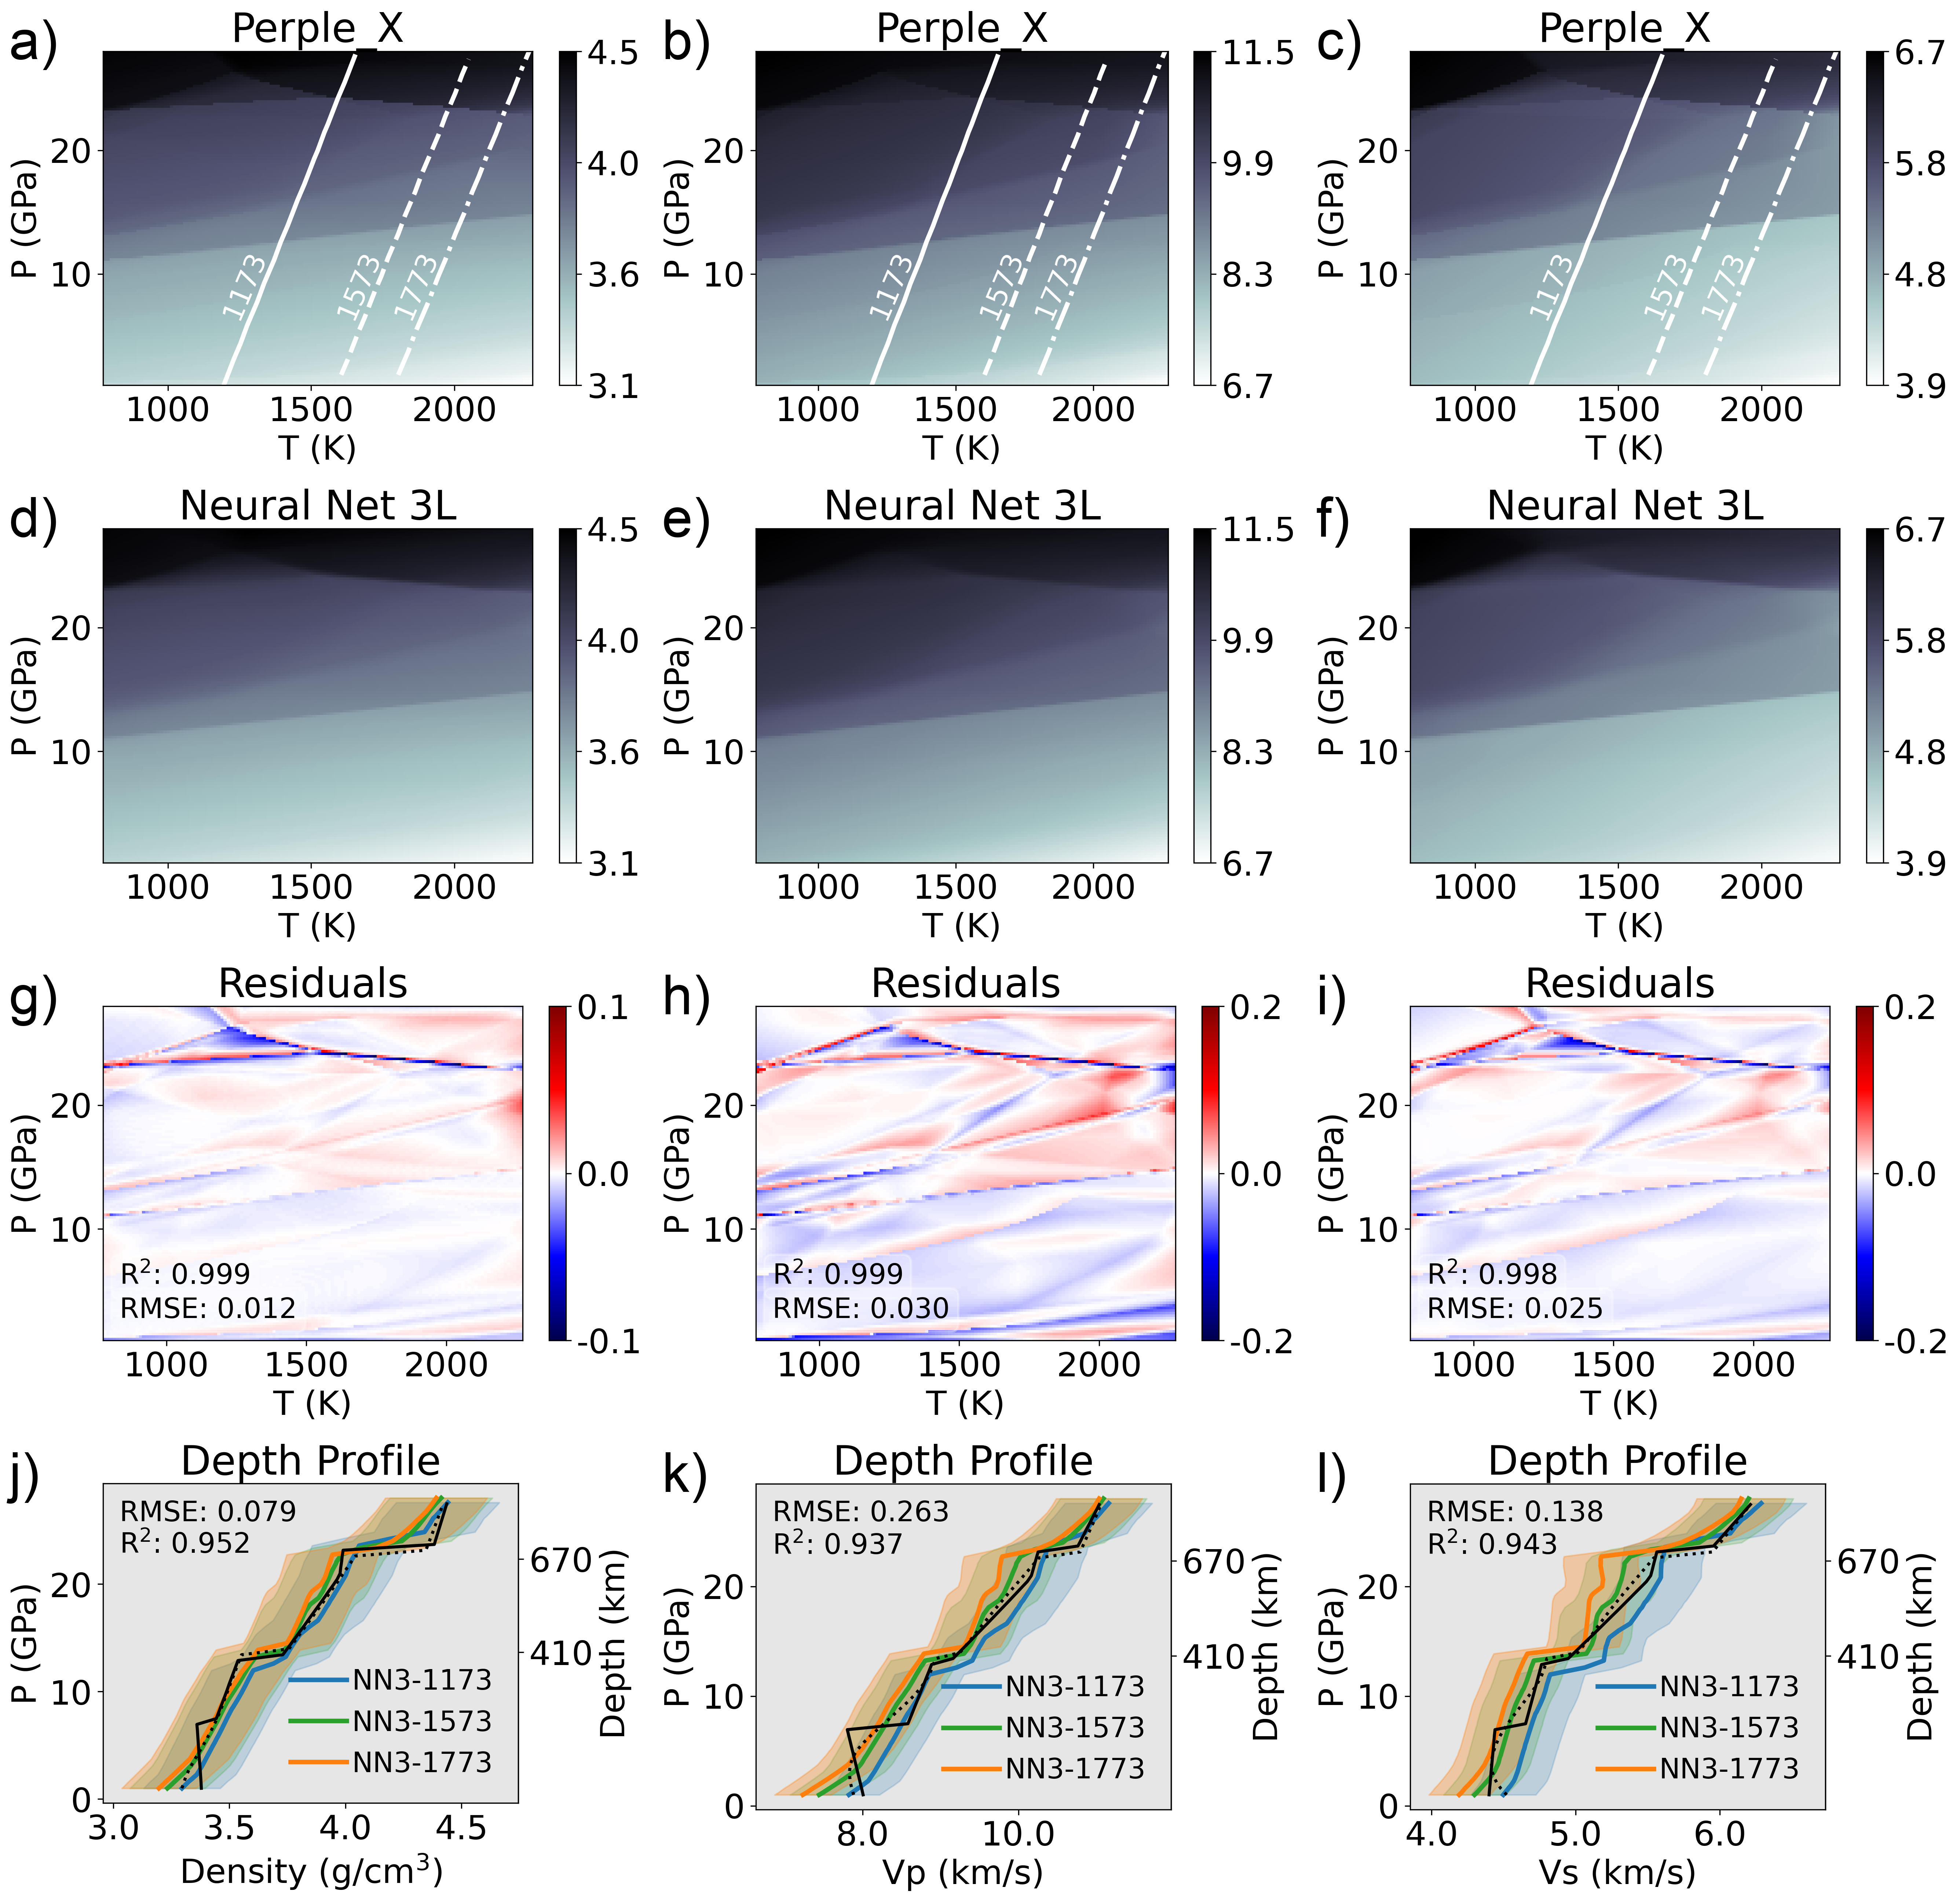
\includegraphics[width=1\linewidth,]{image12-PUM-NN3} 

}

\caption{(ref:image12-PUM-NN3-cap)}\label{fig:image12-PUM-NN3}
\end{figure}

\clearpage

\section*{GFEM, Lookup Table, and RocMLM Performance Datasets}\label{gfem-lookup-table-and-rocmlm-performance-datasets}
\addcontentsline{toc}{section}{GFEM, Lookup Table, and RocMLM Performance Datasets}

The Lookup Table and GFEM performance data referenced in the main text are not included here for brevity, but can be found at \url{https://doi.org/10.17605/OSF.IO/K23TB}. These data are shown in Figure 6 of the main text and referenced in the Introduction of the main text to give a sense of the execution speeds of widely-used GFEM programs (4--228 ms per PTX point). The Introduction of the main text also references a feasibility objective for RocMLM performance (10\(^0\)--10\(^{−1}\) ms), which was estimated with the following reasoning. Numerical geodynamic models on the order of 2000 x 300 km in scale, containing at least 277,221 nodes \citep[921 x 301, e.g.,][]{kerswell2021} are widely-considered ``high-resolution''. Running GFEM on each node (at 4--228 ms/node) would take between 18.5 minutes to 17.5 hours with modern GFEM programs, depending on their configuration and assuming a simple sequential computation. At execution speeds of 10\(^0\)--10\(^{−1}\) ms, however, only 0.5--4.5 minutes of computation time would be added to each timestep, in a similar context. We consider an additional 0.5--4.5 minutes per timestep reasonable considering the advantage of implementing thermodynamic self-consistency in numerical experiments, especially given that parallel computing would further decrease these time estimations. We therefore set 10\(^0\)--10\(^{−1}\) ms as a minimum feasibility objective for RocMLM execution speeds.

Note that Figure 6 of the main text shows a representative subset of the RocMLM performance data evaluated in this study. RocMLM performance was measured multiple times for each regression algorithm: iterating over all combinations of PT and X resolutions (Table \ref{tab:rocmlm-performance}), or model ``capacities'', which was too much data to include in the main text. For graphical clarity, Figure 6 of the main text only shows the set of RocMLM models with the lowest prediction times for each unique model capacity (ranging from 2\(^{11}\)--2\(^{21}\)). The same filtering procedure is equally applied to Lookup Table results. Removing this filtering step (or alternatively selecting for the highest prediction times) does not alter the main conclusions discussed in Section 4 of the main text, but does make the results presented in Figure 6 of the main text easier to digest for the reader. For transparency and reproducibility, the complete RocMLM performance dataset is contained in Table \ref{tab:rocmlm-performance} below.

\begin{longtable}[]{@{}
  >{\raggedright\arraybackslash}p{(\linewidth - 16\tabcolsep) * \real{0.0616}}
  >{\raggedleft\arraybackslash}p{(\linewidth - 16\tabcolsep) * \real{0.1096}}
  >{\raggedleft\arraybackslash}p{(\linewidth - 16\tabcolsep) * \real{0.1027}}
  >{\raggedleft\arraybackslash}p{(\linewidth - 16\tabcolsep) * \real{0.0959}}
  >{\raggedleft\arraybackslash}p{(\linewidth - 16\tabcolsep) * \real{0.1096}}
  >{\raggedleft\arraybackslash}p{(\linewidth - 16\tabcolsep) * \real{0.1575}}
  >{\raggedleft\arraybackslash}p{(\linewidth - 16\tabcolsep) * \real{0.1233}}
  >{\raggedleft\arraybackslash}p{(\linewidth - 16\tabcolsep) * \real{0.1233}}
  >{\raggedleft\arraybackslash}p{(\linewidth - 16\tabcolsep) * \real{0.1164}}@{}}
\caption{\label{tab:rocmlm-performance} RocMLM PTX resolution, accuracy (RMSE vs.~Perple\_X), and performance (training and prediction times) measured on a validation dataset after training.}\tabularnewline
\toprule\noalign{}
\begin{minipage}[b]{\linewidth}\raggedright
Model
\end{minipage} & \begin{minipage}[b]{\linewidth}\raggedleft
PT Res (pts)
\end{minipage} & \begin{minipage}[b]{\linewidth}\raggedleft
X Res (pts)
\end{minipage} & \begin{minipage}[b]{\linewidth}\raggedleft
Train (ms)
\end{minipage} & \begin{minipage}[b]{\linewidth}\raggedleft
Predict (ms)
\end{minipage} & \begin{minipage}[b]{\linewidth}\raggedleft
RMSE rho (g/cm\(^3\))
\end{minipage} & \begin{minipage}[b]{\linewidth}\raggedleft
RMSE Vp (km/s)
\end{minipage} & \begin{minipage}[b]{\linewidth}\raggedleft
RMSE Vs (km/s)
\end{minipage} & \begin{minipage}[b]{\linewidth}\raggedleft
Filesize (Mb)
\end{minipage} \\
\midrule\noalign{}
\endfirsthead
\toprule\noalign{}
\begin{minipage}[b]{\linewidth}\raggedright
Model
\end{minipage} & \begin{minipage}[b]{\linewidth}\raggedleft
PT Res (pts)
\end{minipage} & \begin{minipage}[b]{\linewidth}\raggedleft
X Res (pts)
\end{minipage} & \begin{minipage}[b]{\linewidth}\raggedleft
Train (ms)
\end{minipage} & \begin{minipage}[b]{\linewidth}\raggedleft
Predict (ms)
\end{minipage} & \begin{minipage}[b]{\linewidth}\raggedleft
RMSE rho (g/cm\(^3\))
\end{minipage} & \begin{minipage}[b]{\linewidth}\raggedleft
RMSE Vp (km/s)
\end{minipage} & \begin{minipage}[b]{\linewidth}\raggedleft
RMSE Vs (km/s)
\end{minipage} & \begin{minipage}[b]{\linewidth}\raggedleft
Filesize (Mb)
\end{minipage} \\
\midrule\noalign{}
\endhead
\bottomrule\noalign{}
\endlastfoot
DT & 8 & 2 & 0.77 & 0.03 & 0.017 & 0.038 & 0.038 & 0.034 \\
DT & 8 & 32 & 2.8 & 0.04 & 0.014 & 0.034 & 0.034 & 0.313 \\
DT & 8 & 64 & 5.1 & 0.05 & 0.014 & 0.034 & 0.034 & 0.572 \\
DT & 8 & 128 & 8.5 & 0.05 & 0.014 & 0.034 & 0.034 & 0.52 \\
DT & 16 & 2 & 1.1 & 0.04 & 0.0098 & 0.022 & 0.021 & 0.117 \\
DT & 16 & 32 & 9.7 & 0.04 & 0.013 & 0.029 & 0.027 & 1.12 \\
DT & 16 & 64 & 19 & 0.05 & 0.013 & 0.029 & 0.027 & 2.04 \\
DT & 16 & 128 & 34 & 0.05 & 0.014 & 0.029 & 0.027 & 1.86 \\
DT & 32 & 2 & 3.6 & 0.04 & 0.0099 & 0.022 & 0.02 & 0.44 \\
DT & 32 & 32 & 43 & 0.07 & 0.011 & 0.022 & 0.021 & 4.22 \\
DT & 32 & 64 & 39 & 0.07 & 0.011 & 0.022 & 0.022 & 4.63 \\
DT & 32 & 128 & 170 & 0.09 & 0.011 & 0.022 & 0.022 & 7.02 \\
DT & 64 & 2 & 14 & 0.04 & 0.011 & 0.022 & 0.022 & 1.7 \\
DT & 64 & 32 & 220 & 0.09 & 0.011 & 0.023 & 0.022 & 16.4 \\
DT & 64 & 64 & 440 & 0.11 & 0.012 & 0.023 & 0.022 & 29.8 \\
DT & 64 & 128 & 790 & 0.15 & 0.012 & 0.023 & 0.023 & 27.2 \\
DT & 128 & 2 & 64 & 0.06 & 0.01 & 0.022 & 0.022 & 6.71 \\
DT & 128 & 32 & 1000 & 0.12 & 0.011 & 0.023 & 0.022 & 64.4 \\
DT & 128 & 64 & 2100 & 0.17 & 0.011 & 0.023 & 0.022 & 117 \\
DT & 128 & 128 & 4100 & 0.18 & 0.011 & 0.023 & 0.022 & 108 \\
KN & 8 & 2 & 0.39 & 0.18 & 0.027 & 0.078 & 0.058 & 0.017 \\
KN & 8 & 32 & 0.61 & 0.16 & 0.015 & 0.035 & 0.034 & 0.174 \\
KN & 8 & 64 & 0.98 & 0.16 & 0.015 & 0.035 & 0.034 & 0.342 \\
KN & 8 & 128 & 1.6 & 0.17 & 0.015 & 0.034 & 0.034 & 0.678 \\
KN & 16 & 2 & 0.47 & 0.14 & 0.015 & 0.041 & 0.033 & 0.057 \\
KN & 16 & 32 & 1.5 & 0.17 & 0.014 & 0.031 & 0.028 & 0.603 \\
KN & 16 & 64 & 2.9 & 0.18 & 0.014 & 0.029 & 0.027 & 1.19 \\
KN & 16 & 128 & 6 & 0.23 & 0.014 & 0.029 & 0.027 & 2.35 \\
KN & 32 & 2 & 0.67 & 0.22 & 0.011 & 0.028 & 0.024 & 0.21 \\
KN & 32 & 32 & 7.4 & 0.45 & 0.011 & 0.024 & 0.023 & 2.27 \\
KN & 32 & 64 & 14 & 0.29 & 0.011 & 0.023 & 0.022 & 4.48 \\
KN & 32 & 128 & 31 & 0.31 & 0.011 & 0.023 & 0.022 & 8.89 \\
KN & 64 & 2 & 2.1 & 0.21 & 0.011 & 0.023 & 0.022 & 0.814 \\
KN & 64 & 32 & 29 & 0.3 & 0.012 & 0.024 & 0.023 & 8.82 \\
KN & 64 & 64 & 56 & 0.33 & 0.012 & 0.023 & 0.023 & 17.4 \\
KN & 64 & 128 & 120 & 0.35 & 0.012 & 0.023 & 0.023 & 34.5 \\
KN & 128 & 2 & 8.4 & 0.2 & 0.01 & 0.022 & 0.022 & 3.2 \\
KN & 128 & 32 & 130 & 0.47 & 0.011 & 0.023 & 0.022 & 34.8 \\
KN & 128 & 64 & 270 & 0.62 & 0.011 & 0.023 & 0.022 & 68.5 \\
KN & 128 & 128 & 610 & 0.95 & 0.011 & 0.023 & 0.022 & 136 \\
NN1 & 8 & 2 & 240 & 0.03 & 0.049 & 0.15 & 0.12 & 0.02 \\
NN1 & 8 & 32 & 450 & 0.04 & 0.042 & 0.13 & 0.11 & 0.02 \\
NN1 & 8 & 64 & 13000 & 0.1 & 0.04 & 0.12 & 0.096 & 0.02 \\
NN1 & 8 & 128 & 14000 & 0.09 & 0.035 & 0.09 & 0.077 & 0.02 \\
NN1 & 16 & 2 & 270 & 0.04 & 0.052 & 0.15 & 0.13 & 0.02 \\
NN1 & 16 & 32 & 14000 & 0.13 & 0.036 & 0.087 & 0.081 & 0.02 \\
NN1 & 16 & 64 & 16000 & 0.12 & 0.029 & 0.072 & 0.068 & 0.02 \\
NN1 & 16 & 128 & 32000 & 0.1 & 0.021 & 0.06 & 0.055 & 0.02 \\
NN1 & 32 & 2 & 14000 & 0.07 & 0.04 & 0.12 & 0.099 & 0.02 \\
NN1 & 32 & 32 & 32000 & 0.13 & 0.025 & 0.061 & 0.057 & 0.02 \\
NN1 & 32 & 64 & 51000 & 0.11 & 0.022 & 0.055 & 0.051 & 0.02 \\
NN1 & 32 & 128 & 82000 & 0.16 & 0.019 & 0.05 & 0.046 & 0.02 \\
NN1 & 64 & 2 & 15000 & 0.08 & 0.03 & 0.073 & 0.068 & 0.019 \\
NN1 & 64 & 32 & 84000 & 0.13 & 0.02 & 0.048 & 0.044 & 0.019 \\
NN1 & 64 & 64 & 140000 & 0.11 & 0.016 & 0.039 & 0.039 & 0.019 \\
NN1 & 64 & 128 & 250000 & 0.14 & 0.017 & 0.045 & 0.041 & 0.019 \\
NN1 & 128 & 2 & 36000 & 0.12 & 0.022 & 0.055 & 0.051 & 0.02 \\
NN1 & 128 & 32 & 250000 & 0.1 & 0.017 & 0.041 & 0.038 & 0.02 \\
NN1 & 128 & 64 & 500000 & 0.13 & 0.017 & 0.042 & 0.04 & 0.02 \\
NN1 & 128 & 128 & 980000 & 0.11 & 0.016 & 0.039 & 0.036 & 0.02 \\
NN2 & 8 & 2 & 290 & 0.04 & 0.045 & 0.12 & 0.11 & 0.045 \\
NN2 & 8 & 32 & 14000 & 0.07 & 0.034 & 0.098 & 0.089 & 0.045 \\
NN2 & 8 & 64 & 26000 & 0.13 & 0.024 & 0.076 & 0.072 & 0.045 \\
NN2 & 8 & 128 & 28000 & 0.11 & 0.016 & 0.046 & 0.04 & 0.045 \\
NN2 & 16 & 2 & 14000 & 0.1 & 0.046 & 0.12 & 0.11 & 0.045 \\
NN2 & 16 & 32 & 28000 & 0.1 & 0.017 & 0.056 & 0.046 & 0.045 \\
NN2 & 16 & 64 & 32000 & 0.09 & 0.015 & 0.043 & 0.035 & 0.045 \\
NN2 & 16 & 128 & 63000 & 0.15 & 0.014 & 0.037 & 0.032 & 0.045 \\
NN2 & 32 & 2 & 26000 & 0.11 & 0.033 & 0.088 & 0.079 & 0.045 \\
NN2 & 32 & 32 & 63000 & 0.11 & 0.013 & 0.032 & 0.027 & 0.045 \\
NN2 & 32 & 64 & 96000 & 0.12 & 0.012 & 0.032 & 0.027 & 0.045 \\
NN2 & 32 & 128 & 150000 & 0.14 & 0.013 & 0.037 & 0.033 & 0.045 \\
NN2 & 64 & 2 & 29000 & 0.13 & 0.02 & 0.054 & 0.048 & 0.043 \\
NN2 & 64 & 32 & 160000 & 0.18 & 0.013 & 0.032 & 0.029 & 0.043 \\
NN2 & 64 & 64 & 270000 & 0.15 & 0.011 & 0.03 & 0.026 & 0.043 \\
NN2 & 64 & 128 & 500000 & 0.16 & 0.012 & 0.031 & 0.028 & 0.043 \\
NN2 & 128 & 2 & 67000 & 0.16 & 0.013 & 0.032 & 0.028 & 0.045 \\
NN2 & 128 & 32 & 510000 & 0.15 & 0.012 & 0.028 & 0.025 & 0.045 \\
NN2 & 128 & 64 & 1e+06 & 0.14 & 0.015 & 0.032 & 0.03 & 0.045 \\
NN2 & 128 & 128 & 2.1e+06 & 0.19 & 0.015 & 0.037 & 0.032 & 0.045 \\
NN3 & 8 & 2 & 330 & 0.04 & 0.04 & 0.12 & 0.1 & 0.069 \\
NN3 & 8 & 32 & 27000 & 0.1 & 0.021 & 0.061 & 0.059 & 0.069 \\
NN3 & 8 & 64 & 40000 & 0.11 & 0.016 & 0.048 & 0.044 & 0.069 \\
NN3 & 8 & 128 & 42000 & 0.15 & 0.016 & 0.042 & 0.037 & 0.069 \\
NN3 & 16 & 2 & 27000 & 0.08 & 0.04 & 0.12 & 0.099 & 0.069 \\
NN3 & 16 & 32 & 42000 & 0.16 & 0.015 & 0.048 & 0.039 & 0.069 \\
NN3 & 16 & 64 & 47000 & 0.11 & 0.015 & 0.042 & 0.035 & 0.069 \\
NN3 & 16 & 128 & 91000 & 0.16 & 0.016 & 0.041 & 0.034 & 0.069 \\
NN3 & 32 & 2 & 40000 & 0.2 & 0.028 & 0.072 & 0.067 & 0.069 \\
NN3 & 32 & 32 & 92000 & 0.13 & 0.011 & 0.027 & 0.024 & 0.069 \\
NN3 & 32 & 64 & 140000 & 0.13 & 0.014 & 0.037 & 0.033 & 0.069 \\
NN3 & 32 & 128 & 220000 & 0.13 & 0.012 & 0.03 & 0.026 & 0.069 \\
NN3 & 64 & 2 & 44000 & 0.14 & 0.016 & 0.044 & 0.037 & 0.068 \\
NN3 & 64 & 32 & 230000 & 0.17 & 0.013 & 0.028 & 0.026 & 0.068 \\
NN3 & 64 & 64 & 400000 & 0.14 & 0.012 & 0.027 & 0.025 & 0.068 \\
NN3 & 64 & 128 & 780000 & 0.18 & 0.012 & 0.027 & 0.024 & 0.068 \\
NN3 & 128 & 2 & 97000 & 0.18 & 0.012 & 0.03 & 0.025 & 0.069 \\
NN3 & 128 & 32 & 780000 & 0.15 & 0.011 & 0.025 & 0.023 & 0.069 \\
NN3 & 128 & 64 & 1.6e+06 & 0.12 & 0.011 & 0.025 & 0.023 & 0.069 \\
NN3 & 128 & 128 & 2.9e+06 & 0.16 & 0.012 & 0.025 & 0.024 & 0.069 \\
\end{longtable}

\clearpage

\cleardoublepage

\bibliography{main.bib}


\end{document}
